\chapter{Finite element method}
\label{ch:Finite_element_method}
El calculo variacional es una disciplina que se encarga de encontrar el minimo de un funcional. En donde un funcional es el mapeo de un espacio vectorial a los reales. Si esta es la ecuacion diferencial

Lu = f

Entonces el residuo es

R(v) = Lv - f

y si se evalua en la solucion u

R(u) = 0

entonces minimizar un residio no tiene gracia, porque se trata de encontrar la solucion exacta a la ecuacion diferencial. Que es lo que no sabemos hacer. Pero entonces podemos proponer minimizar un residuo promediado, p. ej., la norma del error. Entonces definimos un residuo ponderado

Rp(u,v) = int(v*Lu - v*f)

(weigthin se dice ponderar en espanhol). Entonces, uno propone una solucion con una forma conocida: senos y cosenos, polinomios, Gaussianas... Y encuentra la combinacion lineal de esas funciones que minimiza Rp (Ya estamos hablando de metodos aproximados para resolver la ecuacion diferencial).

The Finite Element Method approximate an integral formulation that is --in some sense-- equivalent with a differential equation. This integral (weak) formulation could be obtained from a variational principle, such as the Principle of Virtual Works, or the Integral of Action \cite{Goldstein2001}, but could also be obtained from a more general approach like the Weigthed Residue Method \cite{Zienkiewicz2005, Reddy_functional_analysis}. In the cas of electromagnetic waves, we can formulate a variational principle where the functional to be minimized is the energy carried by the electric and magnetic fields note[NGZ]{Falta esta referencia, que ya se mencion\'o en el cap\'itulo anterior}. 

This project uses the Galerkin Finite Element Method to construct an approximate solution of  initial-boundary value problems involving the wave equation of electromagnetic fields \ref{eq:E-wave-harmonic2}.

Galerkin's method converts a continuous operator problem like a differential equation to a discrete problem by stating it as a weighted residual formulation. 

\section{Weak formulation of the problem}\note[NGZ]{Hace falta una buena limpieza de estilo en este cap\'itulo.}

In a weighted residual formulation weight functions 
are used in order to minimize a functional
that is stated as the integral of the operator problem over the simulation domain\ref{fig:domain}. 

\begin{figure}[h]
\centering
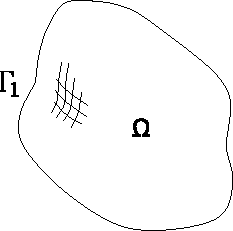
\includegraphics[height=5cm]{./img/dominio.pdf}
\caption{Abstract simulation domain and boundary}
\label{fig:domain}
\end{figure}


Galerkin method involves weight functions that
belong to the same space as the solution.
integration over the domain:

My weight functions wanna be called $\mathbf{W}$ instead. They will belong to the same function space as $\mathbf{E}$.

$\int_{\Omega} \mathbf{W} \cdot$(\ref{eq:E-wave-harmonic2}):

\begin{equation}
\int_{\Omega}\mathbf{W}\cdot\left[ \nabla\times\ \left(\bar{\bar{\mu_r}}^{-1}\nabla\times \mathbf{E} \right) - k_0^{2}\bar{\bar{\epsilon_r}}\cdot \mathbf{E}\right]= - ik_0Z_0 \int_{\Omega} \mathbf{W}\cdot\mathbf{J} \label{eq:E-wave-harmonic3} 
\end{equation}
\begin{equation}
\int_{\Omega}\mathbf{W}\cdot \nabla\times\ \left(\bar{\bar{\mu_r}}^{-1}\nabla\times \mathbf{E} \right) -k_0^{2}\int_{\Omega}\mathbf{W}\cdot \bar{\bar{\epsilon_r}}\cdot \mathbf{E}= - ik_0Z_0 \int_{\Omega} \mathbf{W}\cdot\mathbf{J} \label{eq:E-wave-harmonic3} 
\end{equation}
Now lets focus on the first integral on the left hand side of the equation. Here we will invoke the vector identity: $\mathbf{A}\cdot\nabla\times\mathbf{B} = \mathbf{B}\cdot\nabla\times\mathbf{A} - \nabla\cdot(\mathbf{A}\times\mathbf{B})$ 
Where $\mathbf{A}=\mathbf{W}$ and $\mathbf{B}=\bar{\bar{\epsilon_r}}\nabla\times \mathbf{E}$ To express it as:

\begin{equation}
\int_{\Omega}\mathbf{W}\cdot \nabla\times\ \left(\bar{\bar{\mu_r}}^{-1}\nabla\times \mathbf{E} \right) = \int_{\Omega} \bar{\bar{\mu_r}}^{-1}\nabla\times \mathbf{E}\cdot \nabla\times\mathbf{W}-\int_{\Omega}\nabla\cdot
\left(\mathbf{W}\times\bar{\bar{\mu_r}}^{-1}\nabla\times\mathbf{E}
\right) 
\end{equation}

The Divergence Theorem allows us to transform the volume integral on the second term of the right hand side to a closed surface integral:

\begin{equation}
\int_{\Omega}\nabla\cdot
\left(\mathbf{W}\times\bar{\bar{\mu_r}}^{-1}\nabla\times\mathbf{E}
\right) = \oint_{\Gamma}\hat{n}\cdot
\left(\mathbf{W}\times\bar{\bar{\mu_r}}^{-1}\nabla\times\mathbf{E}
\right) 
\end{equation}

And we will have two kinds of boundaries, Dirichlet and Newman (Reference some textbook), thus $\oint_{\Gamma} = \int_{\Gamma_D}+\int_{\Gamma_N}$. The Dirichlet contribution will be zero because the weight functions  have also been chosen to be zero at Dirichlet boundaries ($\mathbf{W}\mid_{\Gamma_D}=0$). 
One last step is to apply the triple product identity to the argument inside the Newman integral so that:

$$\hat{n}\cdot
\left(\mathbf{W}\times\bar{\bar{\mu_r}}^{-1}
\nabla\times\mathbf{E}\right) =\mathbf{W} \cdot
 \left(\bar{\bar{\mu_r}}^{-1}
\nabla\times\mathbf{E}\times\hat{n}\right) = -\mathbf{W} \cdot
 \left(\hat{n}\times\bar{\bar{\mu_r}}^{-1}
\nabla\times\mathbf{E}\right)$$

Substituting everything:

\begin{equation}
\int_{\Omega} \bar{\bar{\mu_r}}^{-1}\nabla\times \mathbf{E}\cdot \nabla\times\mathbf{W}
-k_0^{2}\mathbf{W}\cdot \bar{\bar{\epsilon_r}}\cdot \mathbf{E}
+ \int_{\Gamma_N} \mathbf{W} \cdot
 \left(\hat{n}\times\bar{\bar{\mu_r}}^{-1}
\nabla\times\mathbf{E}\right)
= -ik_0Z_0 \int_{\Omega} \mathbf{W}\cdot\mathbf{J} \label{eq:E-wave-weak} 
\end{equation}


\section{Boundary conditions}

Look for a nice reference that explain the situation on the boundaries and why is it important to define both the field at the boundary or the ratio of the field at the boundary. Maybe something related to the uniqueness of the solution. Pending to include. 
\begin{align}
\hat{n}\times\mathbf{E}&=\mathbf{P} \quad on \ \Gamma_D\\
\hat{n}\times\left(\bar{\bar{\mu_r}}^{-1}
\nabla\times \mathbf{E}\right) &=\mathbf{K}_N \quad on \ \Gamma_N \label{eq:Robin}
\end{align}
$\mathbf{P}$ is the value for tangential electric field on Dirichlet boundaries $\Gamma_D$, $\eta_r$ is the normalized surface impedance and $\mathbf{K}_N$ is a function that represents boundary sources or electric field flux on $\Gamma_N$. 

Replacing equation \ref{eq:Robin} in \ref{eq:E-wave-weak}:
\begin{equation}
\begin{array}{rcl}
\int_{\Omega} \bar{\bar{\mu_r}}^{-1}\nabla\times \mathbf{E}\cdot \nabla\times\mathbf{W}
-k_0^{2}\mathbf{W}\cdot \bar{\bar{\epsilon_r}}\cdot \mathbf{E}
&=& -ik_0Z_0 \int_{\Omega} \mathbf{W}\cdot\mathbf{J}  \\
&&- \int_{\Gamma_N} \mathbf{W} \cdot\mathbf{K}_N
\end{array}
\end{equation}

\begin{equation}
\begin{array}{rcl}
\int_{\Omega} \bar{\bar{\mu_r}}^{-1}\nabla\times \mathbf{E}\cdot \nabla\times\mathbf{W}
-k_0^{2}\mathbf{W}\cdot \bar{\bar{\epsilon_r}}\cdot \mathbf{E}
&=& -ik_0Z_0 \int_{\Omega} \mathbf{W}\cdot\mathbf{J} \label{eq:E-wave-weak_3} \\
&&- \int_{\Gamma_N} \mathbf{W} \cdot\mathbf{K}_N 
\end{array}
\end{equation}

Using:
$$-\mathbf{W}\cdot\left(\hat{n}\times \left( \hat{n}\times 
\mathbf{E} \right)\right)  = \left(\hat{n}\times \mathbf{W}\right)\cdot\left( \hat{n}\times 
\mathbf{E} \right) $$


\section{Abstract form of the equation}

Time to introduce bi linear operators. These operators are meant to ease mathematical manipulations. Let's do some definitions first:
$\mathbb{V}$ is a vector space of square integrable functions that vanishes at Dirichlet boundaries.

$$ \mathbb{V}=\left\lbrace v\in L^2(a,b):a(v,v)<\infty\wedge v(\Gamma_D)=0\right\rbrace$$
$$L^2 =\left\lbrace v: \Omega \rightarrow \mathbb{R}\quad such \ that\quad \int_{\Omega}v^2d\Omega =0\right\rbrace$$ 

\begin{equation}
\begin{array}{rcl}
      a(\mathbf{W},\mathbf{E})&&:\mathbb{V}\times \mathbb{V}\rightarrow \mathbb{R}\\
      a(\mathbf{W},\mathbf{E})&&= \int\limits_{\Omega}  \bar{\bar{\mu_r}}^{-1}\nabla\times \mathbf{E}\cdot \nabla\times\mathbf{W} d\Omega
\label{eq:a_def}
\end{array}
\end{equation}
\begin{equation}
\begin{array}{rcl}
      m(\mathbf{W},\mathbf{E})&:\mathbb{V}\times \mathbb{V}\rightarrow \mathbb{R}\\
      m(\mathbf{W},\mathbf{E})&= \int\limits_{\Omega} k_0^{2}\mathbf{W}\cdot \bar{\bar{\epsilon_r}}\cdot \mathbf{E} d\Omega
\label{eq:m_def}
\end{array}
\end{equation}

\begin{equation}
\begin{array}{rcl}
      q(\mathbf{W})&:\mathbb{V}\rightarrow \mathbb{R}\\
      q(\mathbf{W})&=\int_{\Gamma_N} \mathbf{W} \cdot\mathbf{K}_N
\label{eq:m_def}
\end{array}
\end{equation}

\begin{equation}
\begin{array}{rcl}
      f(\mathbf{W})&:\mathbb{V}\rightarrow \mathbb{R}\\
      f(\mathbf{W})&=ik_0Z_0 \int_{\Omega} \mathbf{W}\cdot\mathbf{J}
\label{eq:m_def}
\end{array}
\end{equation}
Where $\mathbf{J}$ and $\mathbf{K}_N$ are known field and boundary conditions.

These operators take vectors as inputs and return scalars. 

\begin{equation}
a(\mathbf{W},\mathbf{E}) - m(\mathbf{W},\mathbf{E}) = -f(\mathbf{W})-q(\mathbf{W})
\label{eq:abstract_E_wave}
\end{equation}

\section{Base functions and discretization}
For 2D:
$$\mathbf{E}=E(x,y)_x\hat{a}_x + E(x,y)_y \hat{a}_y $$
The domain will be split in elements defined by relations between nodes (Add a figure and explain better how is it that you split a domain). The approximate solution will be computed using interpolations applied to nodal values. 
Lets say that the set of nodes that represent values of the field in the domain is called $\eta$. On nodes belonging to Dirichlet boundaries we will know the value of the field and it is convenient to split the set of nodes into its known and unknown elements $\eta_D\cup\eta\setminus\eta_D=\eta$.  Each physical node will contain two components of the field, one for $x$ and the other for $y$. So the number of evaluation nodes gets doubled.

If $N$ is the total number of values:

$$N = n_x+ n_y$$.

Where $n_x$ and $n_y$ are the number of evaluation nodes associated to fields in $x$ and  $y$	. When programming it is convenient to distinguish where does a node belongs, so I will treat $n_x$ and $n_y$ as sets as well in order to build a notation for the sums based on  how an iterator surfs a set.

$$n_x = n_x \in \eta_D + n_x \in \eta\setminus\eta_D $$
$$n_y = n_y \in \eta_D + n_y \in \eta\setminus\eta_D $$
If I say: $$i: n_x\in \eta_D$$  That will mean that the iteration will occur on the indexes that belong to the set of nodes in the Dirichlet region associated to $x$ component of the field.

\begin{align*}
E(x,y)_x\approx \sum_{i:\ n_x \in \eta_D} h_i E_i^x+\sum_{i:\ n_x \in \eta\setminus\eta_D} h_i E_i^x \\
E(x,y)_y\approx \sum_{i:\ n_y \in \eta_D}h_iE_i^y+
\sum_{i:\ n_x \in \eta\setminus\eta_D}h_iE_i^y
\end{align*}
 
Left side is known values and right side is unknowns.

In the same way but without knowing $W$ on the boundary:
$$\mathbf{W}=W(x,y)_x\hat{a}_x + W(x,y)_y \hat{a}_y $$
\begin{align*}
W(x,y)_x\approx \sum_{i:\ n_x \in \eta_D} h_i W_i^x+\sum_{i:\ n_x \in \eta\setminus\eta_D} h_i W_i^x \\
W(x,y)_y\approx \sum_{i:\ n_y \in \eta_D}h_iW_i^y+
\sum_{i:\ n_x \in \eta\setminus\eta_D}h_iW_i^y
\end{align*}
I believe that with source terms and boundaries the expansion can be made either with only the known values on nodes, or with interpolation functions such as those before.
Right here I think I will ommit interpolation of $\mathbf{J}$ and $\mathbf{K}_N$.
$$\mathbf{J}=J(x,y)_x\hat{a}_x + J(x,y)_y \hat{a}_y $$

\begin{align*}
J(x,y)_x\approx \sum_{i:\ n_x \in \eta_D}h_i J_i^x+\sum_{i:\ n_x \in \eta\setminus\eta_D}h_i J_i^x \\
J(x,y)_y\approx \sum_{i:\ n_y \in \eta_D}J_i^y+
\sum_{i:\ n_x \in \eta\setminus\eta_D}J_i^y
\end{align*}
$$\mathbf{K}_N=K(x,y)_x\hat{a}_x + K(x,y)_y \hat{a}_y $$
\begin{align*}
K(x,y)_x\approx \sum_{i:\ n_x \in \eta_D}h_i K_i^x+\sum_{i:\ n_x \in \eta\setminus\eta_D} 0 \\
K(x,y)_y\approx \sum_{i:\ n_y \in \eta_D}h_i K_i^y+
\sum_{i:\ n_x \in \eta\setminus\eta_D} 0
\end{align*}

Definition of $h_i$ is left for later because its complicated.

Substitution of $\mathbf{E}$ and $\mathbf{W}$, into \ref{eq:weak-E_complete} is a mess. To make it easier lets use the operators and their nice properties. To be bilinear is to be linear in both arguments, to be linear means to satisfy \href{http://en.wikipedia.org/wiki/Additive_function}{additivity} and \href{http://en.wikipedia.org/wiki/Homogeneous_function}{homogeneity}. An illustration of this:

$$a(\alpha u+\beta v, w)=\alpha a(u,w)+\beta a(v,w)$$

$$a(u,\alpha v+\beta w)=\alpha a(u,v)+\beta a(u,w)$$

The rotational and dot product inside the integrals defined in the abstract forms are linear. A proof which I am pending to do will show that the operators themselves are bi linear.
Also, it remains to be prooved if the following is true:
$$a(u,v) = a(v,u)$$
$$m(u,v) = m(v,u)$$


So the following can happen:

\begin{align}
a\left(W_x,E_x\right)&=& a\left( \sum_{i:\ n_x \in \eta_D} h_i W_i^x, \sum_{j:\ n_x \in \eta_D} h_j E_j^x\right)+a\left(\sum_{i:\ n_x \in \eta\setminus\eta_D} h_i W_i^x,\sum_{j:\ n_x \in \eta\setminus\eta_D} h_j E_j^x\right)\nonumber \\
&=&  \sum_{i:\ n_x \in \eta_D}W_i^x a\left(  h_i , \sum_{j:\ n_x \in \eta_D} h_j E_j^x\right)+\sum_{i:\ n_x \in \eta\setminus\eta_D} W_i^x a\left( h_i,\sum_{j:\ n_x \in \eta\setminus\eta_D} h_j E_j^x\right)\nonumber\\
&=&\sum_{i:\ n_x \in \eta_D}W_i^x \sum_{j:\ n_x \in \eta_D}E_j^x a\left(  h_i ,  h_j \right)+\sum_{i:\ n_x \in \eta\setminus\eta_D} W_i^x \sum_{j:\ n_x \in \eta\setminus\eta_D}  E_j^x a\left( h_i, h_j \right)\nonumber\\
&=& \sum_{j:\ n_x \in \eta_D} a\left(  h_i ,  h_j \right)E_j^x \sum_{i:\ n_x \in \eta_D}W_i^x+\sum_{j:\ n_x \in \eta\setminus\eta_D}   a\left( h_i, h_j \right)E_j^x\sum_{i:\ n_x \in \eta\setminus\eta_D} W_i^x \label{eq:substitution_of_app_fields_in_a}
\end{align}

$$\sum_{j:\ n_x \in \eta_D}E_j^x = \vec{g}_j^x $$
$$\sum_{i:\ n_x \in \eta\setminus\eta_D}W_i^x = \vec{W}^x $$
$$\sum_{j:\ n_x \in \eta\setminus\eta_D}E_j^x = \vec{E}^x $$
$$\vec{g}_i = \vec{g}_j^x+\vec{g}_j^y \qquad j = 1.. N$$
$\vec{g}_j$ is a vector of size $N$ that holds values of $E$ on each Dirichlet boundary node for both $x$, and $y$ components. Vector $\hat{g}_i^y$ follows from a simmilar procedure on $E_y$. It is of importance for me as the one to program to say that: even though the sets defined under the summation are subsets of the set of all nodes, when programming, their associate vectors will span the whole domain. In other words this notation stands for entries to indexes to vectors that may be defined full of zeroes. Or in a different approach: $j$ in $j:\ n_x \in \eta_D$ can be indexes 1 and $N$ meaning that the first and last nodes belong to Dirichlet boundary points on $x$ All other elements of the vector are undefined and hold their initiation value zero.


Changing the indexes i,j and using the definition of \href{http://en.wikipedia.org/wiki/Dot_product}{dot product} in a matrix notation we can translate the abstract form as:

\begin{align*}
a\left(W_x,E_x\right)=&\langle \mathbb{A}\vec{g}^x,\vec{W}^x\rangle
+\langle\mathbb{A}\vec{E}^x,\vec{W}^x\rangle  
\end{align*}

Where A is a matrix whose elements contain the indexed integration over the basis functions $h_i$, and $h_j$, these are known values because we know the form of the functions and can easily calculate the integrals by numerical or analytic means.
$$\mathbb{A} = \mathbb{A}^x+\mathbb{A}^y$$
$$\mathbb{A}^x = \sum_{i,j}^{n_x \in \eta\setminus\eta_D} a(h_i,h_j)+\sum_{i,j}^{n_y \in \eta\setminus\eta_D} a(h_i,h_j)$$

The product $\mathbb{A}^x\vec{g}^x = \vec{d}^x$ will be called the Dirichlet vector.
\begin{align}
a\left(W_x,E_x\right)=&\langle \vec{d}^x,\vec{W}^x\rangle
+\langle\mathbb{A}^x\vec{E}^x,\vec{W}^x\rangle \label{eq:potential_discrete} 
\end{align}

In a very similar way but now substituting the approximate functions into the kinetic operator $m(\mathbf{W},\mathbf{E})$ we get:

\begin{align}
m\left(W_x,E_x\right)=&\langle \mathbb{M}^x\vec{g}^x,\vec{W}^x\rangle
+\langle\mathbb{M}^x\vec{E}^x,\vec{W}^x\rangle\nonumber \\
m\left(W_x,E_x\right)=&\langle \vec{b}^x,\vec{W}^x\rangle
+\langle\mathbb{M}^x\vec{E}^x,\vec{W}^x\rangle \label{eq:kinetic_discrete}
\end{align}

With: $$\mathbb{M}=\mathbb{M}^x+\mathbb{M}^y$$$$\mathbb{M} = \sum_{i,j}^{n_x \in \eta\setminus\eta_D} m(h_i,h_j)+\sum_{i,j}^{n_y \in \eta\setminus\eta_D} m(h_i,h_j)$$

And the same follows with operators $q$ and $f$:

\begin{align}
f(W_x) &= \langle \vec{f}^x, \vec{W^x}\rangle \label{eq:body_source}\\
q(W_x) &= \langle \vec{q}^x, \vec{W^x}\rangle \label{eq:newman}\\
\vec{f}_i^x &= ik_0Z_0\sum_{i:\ n_x \in \eta}\int_{\Omega} h_iJ_i^x\nonumber\\
\vec{q}_i^x&= \sum_{i:\ n_x \in \eta_N}\int_{\Gamma_N} h_iK_i^x \nonumber
\end{align}

Where I introduced a subset of the set $\eta  \setminus \eta_D$ called $\eta_N$ which represents nodes on Newman boundaries.

Substituting definitions: \ref{eq:potential_discrete},\ref{eq:kinetic_discrete}, \ref{eq:newman},  \ref{eq:body_source} in equation \ref{eq:abstract_E_wave}, we get:

\begin{align}
\langle\vec{d}^x,\vec{W}^x\rangle
+\langle\mathbb{A}^x\vec{E}^x,\vec{W}^x\rangle-\langle \vec{b}^x,\vec{W}^x\rangle
-\langle\mathbb{M}^x\vec{E}^x,\vec{W}^x\rangle &= -\langle \vec{f}^x, \vec{W^x}\rangle-\langle \vec{q}^x, \vec{W^x}\rangle \nonumber\\
\langle\mathbb{A}^x\vec{E}^x- \mathbb{M}^x\vec{E}^x,\vec{W}^x \rangle &=\langle \vec{b}^x-\vec{d}^x-\vec{q}^x-\vec{f}^x , \vec{W}^x \rangle
\end{align}

Being $\vec{W}^x$ an arbitrary function, the following linear system of equations appear:
\begin{equation}
\left(\mathbb{A}^x-\mathbb{M}^x\right)\vec{E}^x = \vec{b}^x-\vec{d}^x-\vec{q}^x-\vec{f}^x \label{eq:harmonic_eq_sys_x}
\end{equation}
Similarly and following exactly the same procedure:

\begin{equation}
\left(\mathbb{A}^y-\mathbb{M}^y\right)\vec{E}^y = \vec{b}^y-\vec{d}^y-\vec{q}^y-\vec{f}^y \label{eq:harmonic_eq_sys_y}
\end{equation}

And right now I guess those can be summed. I really don't get why I chose to separate them in the first place. Guess it was in order to make it clear that the components where independent.

So, Matrices and vectors are of the same size ($N$) for both equations, and the places where one has zeros has values in the other. I don't see any impediment to sum  \ref{eq:harmonic_eq_sys_x} and \ref{eq:harmonic_eq_sys_y}:

\begin{equation*}
\left(\mathbb{A}^x-\mathbb{M}^x\right)\vec{E}^x+
\left(\mathbb{A}^y-\mathbb{M}^y\right)\vec{E}^y= \vec{b}-\vec{d}-\vec{q}-\vec{f}
\end{equation*}

A system that I really don't know if can be brought to the form $$\mathbb{K}\vec{E}=\vec{v}$$

Something that I've seen happening in many books is to remove rows and columns associated to Dirichlet positions of E in the matrices and vectors of the equation. This is done because we already know the values of E for those points and their information is already saved in vector $\vec{d}$. I will add the symbol $\setminus D$ before the symbols to note that Dirichlet rows and columns should be deleted.

\begin{equation*}
^{\setminus D}\left[\left(\mathbb{A}^x-\mathbb{M}^x\right)\vec{E}^x+
\left(\mathbb{A}^y-\mathbb{M}^y\right)\vec{E}^y= \vec{b}-\vec{d}-\vec{q}-\vec{f}\right]
\end{equation*}

\section{Vectorial vs scalar formulation}
\section{Edge elements vs Node Elements}
\section{Second order elements, shape functions.}


\section{Numerical integration and Gauss quadrature}



\section{Mass matrices}
¿What is the meaning of Mass matrices in EM?

discrete representation of a continuous distribution of something that multiplies the second time derivative of the field.

Mass matrices are cataloged as consistent or diagonal. Consistent mass matrices use the same shape functions as the ones used to generate the element stiffness matrix. All reference to mass matrices mentioned before, were consistent. \cite{RobertD.Cook1989}
The other way to formulate mass matrices is the lumped mass matrix. Which is made by avoiding the interpolation and simply placing particle masses $m_i$ at nodes $i$ of an element such that $\sum m_i$ is the total element mass. 

The great advantage of lumped mass matrices is that they are diagonal and the solution of the system of equations can be performed in a explicit manner convenient for big computational domains.
However, precision is lost by not stating mass as functions to be interpolated. 

To form a lumped mass matrix one can use the HRZ Lumping scheme 
which consist on the following algorithm \cite{RobertD.Cook1989}:

\begin{enumerate}
\item Compute the diagonal coefficients of the consistent mass matrix.
\item Compute the mass for each element $m$.
\item Compute the trace of the matrix $s$.
\item scale all the diagonal coefficients by multiplying them by the ratio $\frac{m}{s}$.
\end{enumerate}

\section{Explicit formulation}
central-difference method
Aproximates the second order derivative of $\mathbf{E}$ by expanding $\mathbf{E}_{n+1}$ and $\mathbf{E}_{n-1}$  in taylor series about time $n \vartriangle t$:

\begin{equation}
\mathbf{E}_{n+1} = \mathbf{E}_n + \delta t \dot{\mathbf{E}}_n +\frac{\delta t^2}{2} \ddot{\mathbf{E}}_n +\frac{\delta t^3}{6} \dddot{\mathbf{E}}_n+ O(\delta t^4)
\label{eq:2d_taylor_exp1}
\end{equation}
\begin{equation}
\mathbf{E}_{n-1} = \mathbf{E}_n - \delta t \dot{\mathbf{E}}_n +\frac{\delta t^2}{2} \ddot{\mathbf{E}}_n-\frac{\delta t^3}{6} \dddot{\mathbf{E}}_n+ O(\delta t^4)
\label{eq:2d_taylor_exp2}
\end{equation}

Restricting to fourth-order accuracy ($O(\delta t^4)$) and  adding \ref{eq:2d_taylor_exp1} to \ref{eq:2d_taylor_exp2} one can easily solve for $\mathbf{E}_{n+1}$:
\begin{equation}
\ddot{\mathbf{E}}_n = \frac{1}{\delta t^2}\left(\mathbf{E}_{n+1}-2 \mathbf{E}_{n} + \mathbf{E}_{n-1}\right)
\label{eq:central-difference}
\end{equation}
subscript $n$ denotes time $n\delta t$ with $\delta t$ being the selected timestep.

Replacing into our general formulation one gets (fix details):

\begin{equation}
\frac{1}{\delta t^2} \mathbb{M} \mathbf{E}_{n+1} = \frac{1}{\delta t^2}\mathbb{M}\left[2
\mathbf{E}_{n}-\mathbf{E}_{n-1}
\right] \mathbb{A}\mathbf{E}_n 	 
\end{equation}

Nice concluding remarks in page 424 of the book.